\documentclass[11pt,aspectratio=169]{beamer}
% Versión handout (sin transiciones): descomentar y comentar la línea anterior.
% \documentclass[handout,11pt,aspectratio=169]{beamer}
\usepackage[utf8]{inputenc}
\usepackage[T1]{fontenc}
\usepackage[spanish]{babel}
\usepackage{pgfpages}
\usepackage{fancyvrb}
\usepackage{tikz}
\usepackage{pgfplots}
\usepackage{soul}
\usepackage{booktabs}
\usepackage{amsmath}
\usepackage{amssymb}
\usepackage{hyperref}
\usepackage{listings}
\usepackage{xcolor}
\usepackage{graphicx}
\usepackage{array}

\pgfplotsset{compat=1.18}
\usetikzlibrary{arrows.meta,positioning,shapes.geometric,fit,backgrounds,calc,shadows.blur}

% COLORES
\definecolor{blue}{RGB}{0,118,186}
\definecolor{red}{RGB}{181,23,0}
\definecolor{gray}{RGB}{146,146,146}
\definecolor{lightblue}{RGB}{235,244,250}

\definecolor{gray97}{gray}{.97}
\definecolor{gray75}{gray}{.75}
\definecolor{gray45}{gray}{.45}

\lstset{
     frame=Ltb,
     backgroundcolor=\color{gray97},
     basicstyle=\tiny\ttfamily,
     commentstyle=\color{gray45},
     breaklines=true,
     showstringspaces=false,
     columns=fullflexible,
     keepspaces=true,
     literate={á}{{\'a}}1 {é}{{\'e}}1 {í}{{\'i}}1 {ó}{{\'o}}1 {ú}{{\'u}}1 {Á}{{\'A}}1 {É}{{\'E}}1 {Í}{{\'I}}1 {Ó}{{\'O}}1 {Ú}{{\'U}}1 {ñ}{{\~n}}1 {Ñ}{{\~N}}1 {ü}{{\"u}}1 {¿}{{?`}}1 {¡}{{!`}}1,
}

\usetheme{auriga}
\usecolortheme{auriga}

\newcommand{\todo}{\textcolor{red}{\textbf{TODO(alumno)}}}
\newcommand{\code}[1]{\texttt{#1}}

\title{\Large{Laboratorio: Noticias delictuales, LLM y Obsidian\\ \normalsize De texto no estructurado a grafo de conocimiento}}
\subtitle{Business Understanding, Data Understanding, Gemini, JSON y Markdown}
\author{Dr. Juan Bekios Calfa}
\institute[UCN]{\textbf{Machine Learning / Gestión de Proyectos en IA}\\Universidad Católica del Norte}
\date{\textbf{Publicación:} Septiembre 2026 \hspace{1cm} \textbf{Entrega:} Por definir}

\begin{document}

\begin{frame}
\titlepage
\end{frame}

%------------------------------------------------
\begin{frame}{Idea central del laboratorio}
\begin{columns}[T,onlytextwidth]
\column{0.60\textwidth}
\footnotesize
\begin{itemize}[<+->]
\item Los alumnos tomarán noticias delictuales publicadas en Internet.
\item Convertirán texto no estructurado en un JSON con entidades, hechos y relaciones.
\item La persistencia no será una base de datos tradicional.
\item La información final se organizará como una jerarquía de notas Markdown para Obsidian.
\item El resultado esperado es un grafo navegable para analizar relaciones entre delitos, personas, lugares y organizaciones.
\end{itemize}
\column{0.36\textwidth}
\centering
\resizebox{!}{0.66\textheight}{%
\begin{tikzpicture}[font=\scriptsize, node distance=0.50cm]
\node[draw=blue, fill=lightblue, rounded corners=2mm, minimum width=2.55cm, minimum height=0.6cm, align=center] (a) {Noticias};
\node[draw=blue, fill=lightblue, rounded corners=2mm, minimum width=2.55cm, minimum height=0.6cm, below=of a, align=center] (b) {Texto limpio};
\node[draw=blue, fill=lightblue, rounded corners=2mm, minimum width=2.55cm, minimum height=0.6cm, below=of b, align=center] (c) {Gemini};
\node[draw=red, fill=red!10, rounded corners=2mm, minimum width=2.55cm, minimum height=0.6cm, below=of c, align=center] (d) {JSON};
\node[draw=red, fill=red!10, rounded corners=2mm, minimum width=2.55cm, minimum height=0.6cm, below=of d, align=center] (e) {Obsidian};
\draw[-{Latex[length=1.6mm]}, thick, blue] (a)--(b);
\draw[-{Latex[length=1.6mm]}, thick, blue] (b)--(c);
\draw[-{Latex[length=1.8mm]}, thick, red] (c)--(d);
\draw[-{Latex[length=1.8mm]}, thick, red] (d)--(e);
\end{tikzpicture}%
}
\end{columns}
\end{frame}

%------------------------------------------------
\begin{frame}{Pregunta guía}
\small
\begin{block}{Pregunta de trabajo}
¿Cómo transformar noticias delictuales publicadas en Internet en una base de conocimiento estructurada que permita identificar hechos, entidades y relaciones entre delitos?
\end{block}

\vspace{0.25cm}
\begin{alertblock}<2->{Restricción metodológica}
En este laboratorio no se entrenará un modelo de clustering. Los grupos se formarán por relaciones explícitas: mismo delito, misma persona, misma organización, mismo lugar o combinaciones de entidades compartidas.
\end{alertblock}
\end{frame}

%------------------------------------------------
\begin{frame}{Objetivos del laboratorio}
\scriptsize
\begin{block}{Objetivo general}
Construir un pipeline reproducible que capture noticias delictuales, extraiga información relevante con un LLM y genere automáticamente una bóveda de Obsidian para analizar relaciones entre entidades.
\end{block}

\begin{block}<2->{Objetivos específicos}
\begin{itemize}[<+->]
\item Formular el problema desde Business Understanding.
\item Diseñar un modelo de conocimiento: noticias, delitos, personas, organizaciones, lugares y relaciones.
\item Capturar noticias desde fuentes abiertas y preparar texto limpio.
\item Usar Gemini para extraer información en JSON válido.
\item Transformar el JSON en notas Markdown enlazadas.
\item Usar Obsidian para explorar relaciones y agrupamientos simples.
\item Realizar Data Understanding con estadísticas y visualizaciones básicas.
\end{itemize}
\end{block}
\end{frame}

%------------------------------------------------
\begin{frame}{Arquitectura general}
\centering
\resizebox{0.96\linewidth}{!}{%
\begin{tikzpicture}[font=\tiny, node distance=0.55cm,
box/.style={draw=blue, fill=lightblue, rounded corners=2mm, minimum width=2.05cm, minimum height=0.62cm, align=center},
rbox/.style={draw=red, fill=red!10, rounded corners=2mm, minimum width=2.05cm, minimum height=0.62cm, align=center},
arrow/.style={-{Latex[length=1.7mm]}, thick}]
\node[box] (a) {Internet\\Google News};
\node[box, right=0.55cm of a] (b) {URLs\\seleccionadas};
\node[box, right=0.55cm of b] (c) {Captura\\HTML/texto};
\node[box, right=0.55cm of c] (d) {Limpieza\\normalización};
\node[rbox, below=0.85cm of d] (e) {Gemini\\LLM};
\node[rbox, left=0.55cm of e] (f) {JSON\\validado};
\node[rbox, left=0.55cm of f] (g) {Markdown\\automático};
\node[rbox, left=0.55cm of g] (h) {Vault\\Obsidian};
\draw[arrow, blue] (a)--(b);
\draw[arrow, blue] (b)--(c);
\draw[arrow, blue] (c)--(d);
\draw[arrow, red] (d)--(e);
\draw[arrow, red] (e)--(f);
\draw[arrow, red] (f)--(g);
\draw[arrow, red] (g)--(h);
\end{tikzpicture}%
}

\vspace{0.3cm}
\footnotesize
El JSON es un formato intermedio. La persistencia final queda en la jerarquía de archivos de Obsidian.\\
En azul: etapas ya implementadas en el repositorio. En rojo: módulos que el alumno debe completar.
\end{frame}

%------------------------------------------------
\begin{frame}{CRISP-DM adaptado al laboratorio}
\begin{columns}[T,onlytextwidth]
\column{0.52\textwidth}
\scriptsize
\begin{enumerate}[<+->]
\item Comprensión del negocio.
\item Comprensión de los datos.
\item Preparación de los datos.
\item Extracción con LLM.
\item Validación del JSON.
\item Generación de conocimiento en Obsidian.
\item Evaluación del resultado y análisis crítico.
\end{enumerate}

\begin{block}<8->{Mensaje principal}
El laboratorio no comienza con Gemini. Comienza definiendo qué información es útil para analizar un hecho delictual.
\end{block}
\column{0.43\textwidth}
\centering
\resizebox{\linewidth}{!}{%
\begin{tikzpicture}[font=\tiny, every node/.style={align=center}]
\node[draw=blue, fill=lightblue, rounded corners=2mm, minimum width=1.95cm, minimum height=0.62cm] (a) at (0,2.0) {Negocio};
\node[draw=blue, fill=lightblue, rounded corners=2mm, minimum width=1.95cm, minimum height=0.62cm] (b) at (2.2,1.0) {Datos};
\node[draw=blue, fill=lightblue, rounded corners=2mm, minimum width=1.95cm, minimum height=0.62cm] (c) at (2.2,-1.0) {Preparación};
\node[draw=red, fill=red!10, rounded corners=2mm, minimum width=1.95cm, minimum height=0.62cm] (d) at (0,-2.0) {LLM/JSON};
\node[draw=red, fill=red!10, rounded corners=2mm, minimum width=1.95cm, minimum height=0.62cm] (e) at (-2.2,-1.0) {Obsidian};
\node[draw=red, fill=red!10, rounded corners=2mm, minimum width=1.95cm, minimum height=0.62cm] (f) at (-2.2,1.0) {Evaluación};
\draw[-{Latex[length=1.8mm]}, thick, blue] (a) -- (b);
\draw[-{Latex[length=1.8mm]}, thick, blue] (b) -- (c);
\draw[-{Latex[length=1.8mm]}, thick, red] (c) -- (d);
\draw[-{Latex[length=1.8mm]}, thick, red] (d) -- (e);
\draw[-{Latex[length=1.8mm]}, thick, red] (e) -- (f);
\draw[-{Latex[length=1.8mm]}, thick, red] (f) -- (a);
\end{tikzpicture}%
}
\end{columns}
\end{frame}

%------------------------------------------------
\begin{frame}{Business Understanding}
\small
\begin{itemize}[<+->]
\item Se asume el rol de un equipo que apoya a un analista de información delictual.
\item El problema no es guardar noticias, sino convertirlas en conocimiento consultable.
\item La salida debe permitir preguntas como: ¿qué delitos se repiten?, ¿qué comunas aparecen?, ¿qué personas u organizaciones se mencionan juntas?
\end{itemize}

\begin{alertblock}<4->{Entregable de esta etapa}
Una ficha breve con usuario, problema, objetivo, alcance, restricciones éticas y definición de qué se considera una relación útil.
\end{alertblock}
\end{frame}

%------------------------------------------------
\begin{frame}{Preguntas para delimitar el alcance}
\scriptsize
\begin{enumerate}[<+->]
\item ¿Qué tipos de delitos se analizarán?
\item ¿El análisis será nacional, regional o comunal?
\item ¿Qué fuentes de noticias serán permitidas?
\item ¿Cuántas noticias mínimas debe procesar cada grupo?
\item ¿Qué entidades deben extraerse siempre?
\item ¿Cómo se tratarán nombres incompletos o iniciales?
\item ¿Qué información no debe inventar el LLM?
\item ¿Qué significa que dos noticias estén relacionadas?
\end{enumerate}
\end{frame}

%------------------------------------------------
\begin{frame}{Modelo de conocimiento}
\scriptsize
\begin{center}
\begin{tabular}{p{3.0cm}p{7.8cm}}
\toprule
\textbf{Entidad} & \textbf{Descripción} \\
\midrule
Noticia & Documento fuente: título, fecha, fuente, URL y resumen. \\
Delito & Tipo delictual principal o secundario mencionado. \\
Persona & Persona nombrada o referida en la noticia, con rol explícito. \\
Organización & Banda, institución, empresa, tribunal, fiscalía u organismo policial. \\
Lugar & Comuna, ciudad, región, país o punto geográfico. \\
Objeto & Arma, sustancia, vehículo, dinero u otro elemento incautado. \\
Relación & Enlace explícito entre entidades: OPERA\_EN, INVESTIGADO\_POR, DETENIDO\_EN. \\
\bottomrule
\end{tabular}
\end{center}

\begin{block}<2->{Principio}
Extraer solo lo que aparece explícitamente en la noticia. Si falta información, usar \code{null} o listas vacías.
\end{block}
\end{frame}

%------------------------------------------------
\begin{frame}[fragile]{JSON esperado}
\tiny
\begin{lstlisting}[language=Python]
{
  "id_noticia": "N001",
  "titulo": "Operativo policial en La Serena",
  "fecha_publicacion": "2026-08-20",
  "fuente": "Medio de prensa",
  "url": "https://...",
  "resumen": "...",
  "delitos": ["Trafico de drogas"],
  "personas": [
    {"nombre": "Juan Perez", "rol": "imputado"}
  ],
  "organizaciones": ["Los X", "Carabineros"],
  "lugares": ["La Serena", "Region de Coquimbo"],
  "objetos": [
    {"tipo": "sustancia", "nombre": "cocaina", "cantidad": null, "unidad": null}
  ],
  "relaciones": [
    {"origen": "Juan Perez", "tipo": "INVESTIGADO_POR", "destino": "Trafico de drogas"},
    {"origen": "Los X", "tipo": "OPERA_EN", "destino": "La Serena"}
  ]
}
\end{lstlisting}
\end{frame}

%------------------------------------------------
\begin{frame}{Adquisición de noticias}
\small
\begin{itemize}[<+->]
\item Nivel básico: el repositorio entrega una lista semilla en \code{data/urls.csv}.
\item Nivel intermedio: el grupo busca noticias usando Google News o buscadores generales.
\item Nivel avanzado: el grupo ejecuta \code{python main.py descubrir}, que consulta el RSS de Google News.
\end{itemize}

\begin{block}<4->{Recomendación}
Para evitar que el scraping sea el centro del laboratorio, se exige una lista inicial de URLs verificadas. El descubrimiento por RSS \textbf{no scrapea} el HTML de \code{news.google.com}.
\end{block}
\end{frame}

%------------------------------------------------
\begin{frame}[fragile]{Entorno conda}
\small
La administración de paquetes se hace \textbf{solo con conda}. No hay \code{requirements.txt}.

\vspace{0.2cm}
\tiny
\begin{lstlisting}
conda env create -f environment.yml
conda activate lab-noticias-obsidian
python main.py capturar
\end{lstlisting}

\vspace{0.15cm}
\scriptsize
\begin{block}{Dependencias}
conda-forge: \code{requests}, \code{beautifulsoup4}, \code{lxml}, \code{feedparser}, \code{pandas}, \code{matplotlib}, \code{python-dotenv}.\\
La API de Gemini queda bajo \code{pip:} \textbf{dentro} de \code{environment.yml}.
\end{block}
\end{frame}

%------------------------------------------------
\begin{frame}[fragile]{Estructura del proyecto (código modular)}
\footnotesize
\begin{block}{Directorios}
\ttfamily\tiny
ML-2026-02-LAB01/\\
|-- main.py\\
|-- environment.yml\\
|-- data/ urls.csv  consultas.csv  raw/  processed/  json/\\
|-- src/\\
|   |-- pipeline.py\\
|   |-- modelos.py\\
|   |-- adquisicion/   (implementado)\\
|   |-- limpieza/      (implementado)\\
|   |-- extraccion/    (\todo)\\
|   |-- validacion/    (\todo)\\
|   |-- conocimiento/  (\todo)\\
|   `-- analisis/      (\todo)\\
|-- obsidian\_vault/\\
`-- docs/
\end{block}

\scriptsize
No se usan notebooks ni scripts sueltos. El orquestador es \code{main.py}; la lógica vive en clases dentro de \code{src/}.
\end{frame}

%------------------------------------------------
\begin{frame}{Diseño POO}
\centering
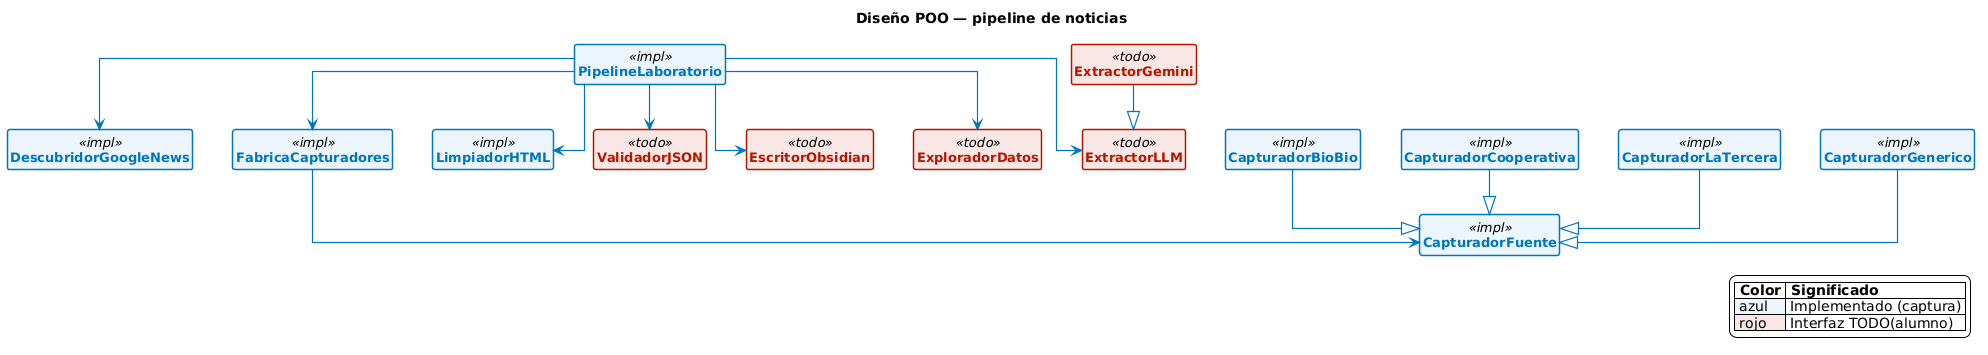
\includegraphics[width=0.98\linewidth,height=0.78\textheight,keepaspectratio]{diseno-poo.png}
\par\scriptsize Azul: implementado (captura). Rojo: interfaz \todo.
\end{frame}

%------------------------------------------------
\begin{frame}[fragile]{Archivo de URLs y consultas}
\tiny
\begin{lstlisting}
# data/urls.csv
id_noticia,fuente,url,categoria_busqueda
N001,BioBioChile,https://...,homicidio
N002,Cooperativa,https://...,trafico_drogas
N003,LaTercera,https://...,homicidio

# data/consultas.csv
consulta,categoria_busqueda,limite
homicidio Chile,homicidio,5
trafico de drogas Chile,trafico_drogas,5
\end{lstlisting}

\scriptsize
\begin{block}<2->{Trazabilidad}
Cada noticia debe mantener su identificador durante todo el pipeline: HTML, texto limpio, JSON y nota Markdown.
\end{block}
\end{frame}

%------------------------------------------------
\begin{frame}[fragile]{Google News: descubrimiento por RSS}
\tiny
\begin{lstlisting}[language=Python]
class DescubridorGoogleNews:
    """No scrapea news.google.com: usa el RSS publico de Chile."""

    def buscar(self, consulta, limite=5):
        params = {"q": consulta, "hl": "es-419",
                  "gl": "CL", "ceid": "CL:es-419"}
        feed = feedparser.parse(GOOGLE_NEWS_RSS + "?" + urlencode(params))
        return list(feed.entries)[:limite]

    def resolver_url_final(self, link_google):
        return self.cliente.url_final(link_google)

    def actualizar_urls_csv(self, consultas=None):
        # Deduplica por URL y asigna id_noticia N00X.
        ...
\end{lstlisting}

\scriptsize
\begin{alertblock}{Uso académico}
Pausa entre peticiones, timeout y User-Agent identificable. Si un redirect falla, se registra el error y el lote continúa.
\end{alertblock}
\end{frame}

%------------------------------------------------
\begin{frame}[fragile]{Captura OOP: fábrica y adaptadores}
\tiny
\begin{lstlisting}[language=Python]
class CapturadorFuente(ABC):
    def acepta(self, url, fuente=None) -> bool: ...
    def obtener_html(self, url) -> str: ...
    def extraer_cuerpo(self, html) -> str: ...

class FabricaCapturadores:
    def para(self, url, fuente=None) -> CapturadorFuente:
        for capturador in self._especificos:  # BioBio, Cooperativa, La Tercera
            if capturador.acepta(url, fuente):
                return capturador
        return self.generico  # fallback
\end{lstlisting}

\scriptsize
\begin{block}{Fallback}
Si el selector CSS del medio no encuentra el artículo, \code{PipelineLaboratorio} usa \code{CapturadorGenerico} (BeautifulSoup).
\end{block}
\end{frame}

%------------------------------------------------
\begin{frame}[fragile]{Limpieza: clase \texttt{LimpiadorHTML}}
\tiny
\begin{lstlisting}[language=Python]
class LimpiadorHTML:
    ETIQUETAS_RUIDO = ("script", "style", "nav", "footer", "aside")
    LARGO_MINIMO_LINEA = 40

    def limpiar(self, html: str) -> str:
        soup = BeautifulSoup(html, "lxml")
        for etiqueta in soup(list(self.ETIQUETAS_RUIDO)):
            etiqueta.decompose()
        lineas = [ln.strip() for ln in soup.get_text("\n").splitlines()]
        lineas = [ln for ln in lineas if len(ln) > self.LARGO_MINIMO_LINEA]
        return "\n".join(lineas)
\end{lstlisting}

\scriptsize
\begin{alertblock}{Cuidado}
El grupo debe respetar términos de uso del sitio, evitar sobrecargar servidores y documentar de dónde obtuvo los textos.
\end{alertblock}
\end{frame}

%------------------------------------------------
\begin{frame}{De HTML a texto útil}
\begin{columns}[T,onlytextwidth]
\column{0.47\textwidth}
\begin{block}{RAW}
\scriptsize
HTML completo, menús, publicidad, recomendaciones, scripts, pie de página y contenido duplicado.
\end{block}
\column{0.47\textwidth}
\begin{alertblock}{Texto limpio}
\scriptsize
Título, fecha, fuente y cuerpo de la noticia en texto plano, listo para ser enviado al LLM.
\end{alertblock}
\end{columns}

\vspace{0.25cm}
\scriptsize
\begin{center}
\begin{tikzpicture}[font=\scriptsize]
\node[draw=blue, fill=lightblue, rounded corners=2mm, minimum width=2.4cm, minimum height=0.7cm] (a) at (0,0) {HTML};
\node[draw=blue, fill=white, rounded corners=2mm, minimum width=2.4cm, minimum height=0.7cm] (b) at (3.0,0) {Limpieza};
\node[draw=red, fill=red!10, rounded corners=2mm, minimum width=2.4cm, minimum height=0.7cm] (c) at (6.0,0) {Texto útil};
\draw[-{Latex[length=1.8mm]}, thick, blue] (a)--(b);
\draw[-{Latex[length=1.8mm]}, thick, red] (b)--(c);
\end{tikzpicture}
\end{center}
\end{frame}

%------------------------------------------------
\begin{frame}[fragile]{Prompt base para Gemini}
\tiny
\begin{lstlisting}
Analiza la siguiente noticia delictual.

Extrae solamente informacion explicita. No inventes datos.
Devuelve exclusivamente JSON valido, sin explicaciones.

Campos obligatorios:
- id_noticia, titulo, fecha_publicacion, fuente, url, resumen
- delitos, personas (nombre y rol), organizaciones, lugares
- objetos, relaciones (origen, tipo, destino)

Si un dato no aparece, usa null o una lista vacia.

NOTICIA:
{{texto_noticia}}
\end{lstlisting}

\scriptsize
\begin{block}<2->{Idea para discusión}
Comparar dos prompts: uno libre y uno con esquema estricto. Evaluar cuál produce JSON más consistente.
\end{block}
\end{frame}

%------------------------------------------------
\begin{frame}[fragile]{Gemini: interfaz para el alumno}
\tiny
\begin{lstlisting}[language=Python]
class ExtractorGemini(ExtractorLLM):
    """TODO(alumno): completar construir_prompt y extraer."""

    def construir_prompt(self, noticia: NoticiaFuente) -> str:
        raise EtapaPendienteAlumno(
            modulo="ExtractorGemini.construir_prompt",
            pista="Prompt estricto + texto de data/processed/{id}.txt",
        )

    def extraer(self, noticia: NoticiaFuente) -> dict:
        # Cargar GEMINI_API_KEY desde .env
        # Llamar a gemini-1.5-flash y guardar data/json/{id}.json
        raise EtapaPendienteAlumno(...)
\end{lstlisting}

\scriptsize
\begin{alertblock}{Importante}
La clave API no debe subirse a GitHub. Usar variables de entorno o archivo \code{.env} excluido por \code{.gitignore}.
\end{alertblock}
\end{frame}

%------------------------------------------------
\begin{frame}[fragile]{Validación del JSON: interfaz}
\tiny
\begin{lstlisting}[language=Python]
class ValidadorJSON:
    CAMPOS_OBLIGATORIOS = [
        "id_noticia", "titulo", "fecha_publicacion", "fuente", "url",
        "resumen", "delitos", "personas", "organizaciones",
        "lugares", "objetos", "relaciones"
    ]

    def validar(self, ruta):
        # TODO(alumno): json.loads + campos faltantes + tipos
        raise EtapaPendienteAlumno(...)
\end{lstlisting}

\scriptsize
\begin{block}{Contrato de datos}
El LLM no es la fuente de verdad. El código debe verificar que su salida cumpla el esquema esperado.
\end{block}
\end{frame}

%------------------------------------------------
\begin{frame}{Obsidian como persistencia}
\small
\begin{itemize}[<+->]
\item No se usará SQLite, MongoDB ni Neo4j.
\item La persistencia final serán archivos Markdown enlazados.
\item Cada noticia y cada entidad relevante tendrá su propia nota.
\item Las relaciones se expresarán mediante enlaces \code{[[...]]} y se visualizarán en el grafo de Obsidian.
\end{itemize}

\begin{alertblock}<5->{Cambio clave}
El sistema no guarda filas en una base de datos. Guarda conocimiento como una red de notas conectadas.
\end{alertblock}
\end{frame}

%------------------------------------------------
\begin{frame}[fragile]{Jerarquía del vault}
\footnotesize
\begin{block}{Estructura esperada}
\ttfamily\tiny
obsidian\_vault/\\
|-- 00\_Indice.md\\
|-- Noticias/\\
|   |-- N001.md\\
|   |-- N002.md\\
|   `-- N003.md\\
|-- Delitos/\\
|   |-- Trafico\_de\_drogas.md\\
|   `-- Homicidio.md\\
|-- Personas/\\
|-- Organizaciones/\\
|-- Lugares/\\
|-- Objetos/\\
`-- Relaciones/\\
\end{block}

\scriptsize
La estructura de carpetas es parte del resultado evaluado.
\end{frame}

%------------------------------------------------
\begin{frame}[fragile]{Nota Markdown de una noticia}
\tiny
\begin{lstlisting}
---
id: N001
fecha_publicacion: 2026-08-20
fuente: Medio de prensa
url: https://...
---

# Operativo policial en La Serena

## Resumen
Texto breve generado desde el JSON.

## Delitos
- [[Trafico de drogas]]

## Personas
- [[Juan Perez]] - imputado

## Organizaciones
- [[Los X]]

## Lugares
- [[La Serena]]

## Relaciones
- [[Juan Perez]] -- INVESTIGADO_POR --> [[Trafico de drogas]]
- [[Los X]] -- OPERA_EN --> [[La Serena]]
\end{lstlisting}
\end{frame}

%------------------------------------------------
\begin{frame}[fragile]{Generar nombres seguros de archivo}
\tiny
\begin{lstlisting}[language=Python]
# Ya implementado en src/conocimiento/utilidades.py
def slugify(text):
    text = unicodedata.normalize("NFKD", text)
    text = "".join(c for c in text if not unicodedata.combining(c))
    text = re.sub(r"[^a-zA-Z0-9]+", "_", text)
    return text.strip("_") or "sin_nombre"

slugify("Tráfico de drogas")       # Trafico_de_drogas
\end{lstlisting}

\scriptsize
\begin{block}{Motivo}
Los nombres de archivos deben ser estables y consistentes para que los enlaces de Obsidian no se rompan. El alumno debe usar esta función al completar el escritor.
\end{block}
\end{frame}

%------------------------------------------------
\begin{frame}[fragile]{Obsidian: interfaz para el alumno}
\tiny
\begin{lstlisting}[language=Python]
class EscritorVaultObsidian(EscritorObsidian):
    def escribir_noticia(self, data: dict) -> Path:
        # TODO(alumno): plantilla Markdown con [[enlaces]]
        raise EtapaPendienteAlumno(...)

    def escribir_entidades(self, noticias: list[dict]) -> None:
        # TODO(alumno): una nota por delito, persona, lugar, ...
        raise EtapaPendienteAlumno(...)

    def escribir_vault(self, noticias: list[dict]) -> None:
        # TODO(alumno): orquestar noticia + entidades + 00_Indice.md
        raise EtapaPendienteAlumno(...)
\end{lstlisting}

\scriptsize
\begin{alertblock}{Persistencia}
La salida final es un archivo \code{.md} dentro de la bóveda de Obsidian, no un JSON suelto.
\end{alertblock}
\end{frame}

%------------------------------------------------
\begin{frame}{Notas de entidades}
\small
Además de las noticias, el laboratorio debe generar notas para las entidades.

\vspace{0.2cm}
\begin{columns}[T,onlytextwidth]
\column{0.47\textwidth}
\begin{block}{Ejemplo: Delito}
\scriptsize
\code{Delitos/Trafico\_de\_drogas.md}
\begin{itemize}
\item Noticias relacionadas.
\item Personas asociadas.
\item Organizaciones mencionadas.
\item Lugares donde aparece.
\end{itemize}
\end{block}
\column{0.47\textwidth}
\begin{alertblock}{Ejemplo: Persona}
\scriptsize
\code{Personas/Juan\_Perez.md}
\begin{itemize}
\item Noticias donde aparece.
\item Rol observado.
\item Delitos asociados.
\item Organizaciones relacionadas.
\end{itemize}
\end{alertblock}
\end{columns}
\end{frame}

%------------------------------------------------
\begin{frame}[fragile]{Nota de entidad: delito}
\tiny
\begin{lstlisting}
# Trafico de drogas

Tipo: Delito

## Noticias relacionadas
- [[N001]]
- [[N007]]
- [[N015]]

## Personas relacionadas
- [[Juan Perez]]
- [[Pedro Soto]]

## Organizaciones relacionadas
- [[Los X]]

## Lugares
- [[La Serena]]
- [[Coquimbo]]
\end{lstlisting}
\end{frame}

%------------------------------------------------
\begin{frame}[fragile]{Construir índices de entidades}
\tiny
\begin{lstlisting}[language=Python]
from collections import defaultdict

indice_delitos = defaultdict(set)
indice_personas = defaultdict(set)
indice_lugares = defaultdict(set)

for data in noticias_json:
    nid = data["id_noticia"]
    for delito in data["delitos"]:
        indice_delitos[delito].add(nid)
    for persona in data["personas"]:
        indice_personas[persona["nombre"]].add(nid)
    for lugar in data["lugares"]:
        indice_lugares[lugar].add(nid)
\end{lstlisting}

\scriptsize
\begin{block}{Idea}
Los índices permiten escribir automáticamente las notas de delitos, personas y lugares sin usar una base de datos. Incorpórelos en \code{escribir\_entidades}.
\end{block}
\end{frame}

%------------------------------------------------
\begin{frame}{Relaciones y agrupamientos simples}
\small
\begin{itemize}[<+->]
\item Un grupo de noticias puede formarse porque comparte el mismo tipo de delito.
\item También puede formarse porque comparte una persona, organización, comuna o institución.
\item Obsidian permite visualizar esas conexiones sin entrenar un algoritmo de clustering.
\end{itemize}

\begin{center}
\resizebox{0.75\linewidth}{!}{%
\begin{tikzpicture}[font=\scriptsize]
\node[draw=red, fill=red!10, rounded corners=2mm] (d) at (0,0) {Tráfico de drogas};
\node[draw=blue, fill=lightblue, rounded corners=2mm] (n1) at (-3,1.1) {N001};
\node[draw=blue, fill=lightblue, rounded corners=2mm] (n2) at (-3,-1.1) {N007};
\node[draw=blue, fill=lightblue, rounded corners=2mm] (n3) at (3,1.1) {N015};
\node[draw=blue, fill=lightblue, rounded corners=2mm] (l) at (3,-1.1) {La Serena};
\draw[-{Latex[length=1.8mm]}, thick, blue] (n1)--(d);
\draw[-{Latex[length=1.8mm]}, thick, blue] (n2)--(d);
\draw[-{Latex[length=1.8mm]}, thick, blue] (n3)--(d);
\draw[-{Latex[length=1.8mm]}, thick, red] (d)--(l);
\end{tikzpicture}%
}
\end{center}
\end{frame}

%------------------------------------------------
\begin{frame}{Data Understanding}
\scriptsize
Una vez generado el corpus estructurado, cada grupo debe analizar sus propios datos.

\vspace{0.15cm}
\begin{columns}[T,onlytextwidth]
\column{0.48\textwidth}
\begin{block}{Preguntas mínimas}
\begin{itemize}
\item ¿Cuántas noticias fueron procesadas?
\item ¿Cuántas fallaron?
\item ¿Qué fuentes fueron usadas?
\item ¿Qué delitos aparecen con mayor frecuencia?
\item ¿Qué lugares concentran más menciones?
\end{itemize}
\end{block}
\column{0.48\textwidth}
\begin{alertblock}{Calidad de datos}
\begin{itemize}
\item Porcentaje de campos nulos.
\item Noticias duplicadas.
\item JSON inválidos.
\item Entidades con nombres inconsistentes.
\item Relaciones dudosas generadas por el LLM.
\end{itemize}
\end{alertblock}
\end{columns}
\end{frame}

%------------------------------------------------
\begin{frame}[fragile]{Análisis: interfaz \texttt{ExploradorDatos}}
\tiny
\begin{lstlisting}[language=Python]
class ExploradorDatos:
    def noticias_por_fuente(self): ...   # TODO(alumno)
    def delitos_frecuentes(self): ...    # TODO(alumno)
    def lugares_frecuentes(self): ...    # TODO(alumno)
    def campos_faltantes(self): ...      # TODO(alumno)
    def evolucion_temporal(self): ...    # TODO(alumno)

    def ejecutar(self):
        # pandas + matplotlib sobre data/json/*.json
        raise EtapaPendienteAlumno(...)
\end{lstlisting}

\scriptsize
La visualización no es decoración. Debe apoyar la comprensión de los datos y revelar problemas de calidad.
\end{frame}

%------------------------------------------------
\begin{frame}{Visualizaciones esperadas}
\small
\begin{itemize}[<+->]
\item Noticias por fuente.
\item Noticias por tipo de delito.
\item Delitos por comuna o región.
\item Cantidad de personas u organizaciones por noticia.
\item Porcentaje de campos faltantes en el JSON.
\item Evolución temporal simple si la fecha está disponible.
\end{itemize}

\begin{alertblock}<7->{Importante}
Interprete cada gráfico en el informe: qué dice sobre cobertura, sesgo o calidad.
\end{alertblock}
\end{frame}

%------------------------------------------------
\begin{frame}{Control de calidad del LLM}
\scriptsize
\begin{center}
\begin{tabular}{p{3.6cm}p{7.0cm}}
\toprule
\textbf{Problema posible} & \textbf{Cómo detectarlo} \\
\midrule
Inventa entidades & Comparar manualmente una muestra de noticias contra el JSON. \\
Confunde roles & Revisar si diferencia víctima, imputado, detenido, fiscal, testigo. \\
Normaliza mal nombres & Crear lista de equivalencias o corregir manualmente. \\
Produce JSON inválido & Usar \code{json.loads} y registrar fallos. \\
Extrae relaciones dudosas & Exigir que cada relación esté respaldada por el texto. \\
\bottomrule
\end{tabular}
\end{center}

\begin{block}<2->{Muestra de auditoría}
Cada grupo debe revisar manualmente al menos 10 noticias procesadas.
\end{block}
\end{frame}

%------------------------------------------------
\begin{frame}{Ética y uso responsable}
\small
\begin{itemize}[<+->]
\item Las noticias pueden contener acusaciones, investigaciones o información sensible.
\item El sistema no debe afirmar culpabilidad si la noticia no lo indica explícitamente.
\item Los roles deben registrarse con cuidado: detenido, imputado, acusado, condenado, víctima o testigo no son equivalentes.
\item Se debe citar la fuente original y conservar la URL.
\item El análisis es académico y exploratorio.
\end{itemize}
\end{frame}

%------------------------------------------------
\begin{frame}{Entregables}
\small
\begin{itemize}[<+->]
\item Repositorio GitHub del laboratorio.
\item Código modular en \code{src/} y orquestador \code{main.py} (sin notebooks).
\item Carpeta \code{data/} con URLs, texto procesado y JSON generado.
\item Carpeta \code{obsidian\_vault/} funcionando en Obsidian.
\item Visualizaciones de Data Understanding.
\item Informe breve con problema, metodología, resultados, errores del LLM y análisis de relaciones.
\end{itemize}
\end{frame}

%------------------------------------------------
\begin{frame}{Pauta de evaluación propuesta}
\small
\begin{center}
\begin{tabular}{p{8.2cm}r}
\toprule
\textbf{Criterio} & \textbf{\%} \\
\midrule
Business Understanding y alcance del problema & 10 \\
Diseño del modelo de conocimiento y JSON & 15 \\
Adquisición y limpieza de noticias & 15 \\
Extracción con Gemini y validación del JSON & 20 \\
Generación automática del vault de Obsidian & 20 \\
Data Understanding y visualizaciones & 10 \\
Análisis crítico, ética y reproducibilidad & 10 \\
\bottomrule
\end{tabular}
\end{center}
\end{frame}

%------------------------------------------------
\begin{frame}{Errores comunes}
\scriptsize
\begin{itemize}[<+->]
\item Guardar solo el JSON y no generar notas enlazadas.
\item Usar Obsidian como carpeta de archivos, pero sin enlaces \code{[[...]]}.
\item Pedirle al LLM análisis libre en lugar de un JSON con esquema definido.
\item No validar la salida del LLM.
\item Mezclar datos inventados con datos extraídos explícitamente.
\item No mantener trazabilidad entre URL, texto, JSON y Markdown.
\item Presentar gráficos sin interpretar qué dicen sobre los datos.
\item Entregar notebooks o scripts sueltos en lugar de clases en \code{src/}.
\end{itemize}
\end{frame}

%------------------------------------------------
\begin{frame}{Resultados esperados de aprendizaje}
\small
Al finalizar el laboratorio, el estudiante debería ser capaz de:
\begin{itemize}[<+->]
\item Formular un problema de análisis de información no estructurada.
\item Diseñar un esquema JSON para extracción de información.
\item Preparar texto de noticias para ser procesado por un LLM.
\item Validar respuestas generadas por un modelo generativo.
\item Convertir información estructurada en una base de conocimiento Markdown.
\item Usar Obsidian para explorar relaciones y patrones simples.
\item Evaluar críticamente la calidad de los datos extraídos.
\end{itemize}
\end{frame}

%------------------------------------------------
\begin{frame}{Secuencia sugerida de trabajo}
\scriptsize
\begin{enumerate}[<+->]
\item Definir alcance: delitos, región, fuentes y tamaño mínimo del corpus.
\item Crear el entorno: \code{conda env create -f environment.yml}.
\item Completar o ampliar \code{data/consultas.csv} y \code{data/urls.csv}.
\item Ejecutar \code{python main.py descubrir} y \code{python main.py capturar}.
\item Completar \code{ExtractorGemini} y el validador JSON.
\item Completar \code{EscritorVaultObsidian} y abrir el vault en Obsidian.
\item Corregir nombres inconsistentes.
\item Completar \code{ExploradorDatos} y el análisis crítico.
\end{enumerate}
\end{frame}

%------------------------------------------------
\begin{frame}[fragile]{Comandos del orquestador}
\tiny
\begin{lstlisting}
python main.py descubrir   # Google News RSS -> data/urls.csv
python main.py capturar    # URLs -> data/raw + data/processed
python main.py extraer     # TODO(alumno) Gemini
python main.py obsidian    # TODO(alumno) vault Markdown
python main.py analizar    # TODO(alumno) Data Understanding
python main.py pipeline    # descubrir + capturar; avisa pendientes
\end{lstlisting}

\scriptsize
Si una etapa \todo{} se invoca sin completar, el programa imprime una pista y \textbf{no falla en silencio}.
\end{frame}

%------------------------------------------------
\begin{frame}{Cierre del laboratorio}
\begin{columns}[T,onlytextwidth]
\column{0.58\textwidth}
\small
\begin{itemize}[<+->]
\item El valor del laboratorio está en el pipeline completo.
\item El LLM ayuda a estructurar, pero no reemplaza la validación humana.
\item Obsidian permite convertir datos extraídos en conocimiento navegable.
\item Las relaciones emergen desde entidades compartidas, no desde un algoritmo de clustering.
\end{itemize}

\column{0.34\textwidth}
\centering
\resizebox{\linewidth}{!}{%
\begin{tikzpicture}[every node/.style={font=\tiny}]
\node[draw=blue, rounded corners=2mm, fill=lightblue, minimum width=2.6cm, minimum height=0.55cm] (t1) at (0,1.5) {Texto no estructurado};
\node[draw=blue, rounded corners=2mm, fill=white, minimum width=2.6cm, minimum height=0.55cm] (t2) at (0,0.2) {JSON validado};
\node[draw=red, rounded corners=2mm, fill=red!8, minimum width=2.6cm, minimum height=0.55cm] (t3) at (0,-1.1) {Grafo en Obsidian};
\draw[-{Latex[length=1.8mm]}, thick, blue] (t1)--(t2);
\draw[-{Latex[length=1.8mm]}, thick, red] (t2)--(t3);
\end{tikzpicture}%
}
\end{columns}
\end{frame}

%------------------------------------------------
\begin{frame}
\centering
\Huge ¿Preguntas?
\end{frame}

\end{document}
